\scanpage{118}
\deleted{dans un \unsure{trou} (\unsure{suivant qu'on est dans le cas indiqué en} $\unsure{R,R}$) les \unsure{tracés gênants}

\figure{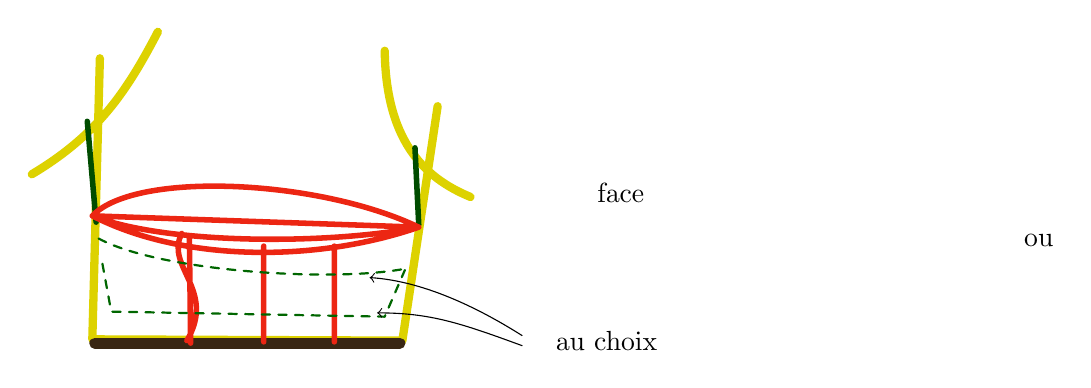
\begin{tikzpicture}[x=.016cm,y=-.016cm,line cap=round,line join=round]
\draw[yellow!70!olive,line width=3pt] (261,386)--(255,609)--(501,610)--(529,424) (207,478)..controls(259,447)and(282,413)..(307,365) (487,380)..controls(488,449)and(516,480)..(555,496);
\draw[black!70!green,line width=2pt] (251,436)--(258,516) (511,457)--(514,518);
\draw[black!70!brown,line width=4pt] (257,612)--(499,612);
\draw[red!70!brown,line width=2pt] (255,511)..controls(289,475)and(435,482)..(514,520)..controls(433,548)and(327,548)..(255,511) (255,511)--(514,520) (255,511)..controls(314,534)and(442,534)..(514,520) (326,525)..controls(312,551)and(354,570)..(330,610) (332,528)--(333,612) (391,535)--(391,611) (447,535)--(447,611);
\draw[black!60!green,thick,dashed] (260,529)..controls(308,555)and(445,564)..(503,553) (263,549)--(270,587)--(487,591)--(503,554);
\draw[->] (596,606)..controls(547,575)and(507,562)..(475,560);\draw[->] (596,614)..controls(547,596)and(523,588)..(481,588);
\node[anchor=west] at (615,610) {au choix};\node[anchor=west] at (648,493) {\deleted{\unsure{face}}};\node at (1006,531) {\unsure{ou}};
\end{tikzpicture}}

\figure{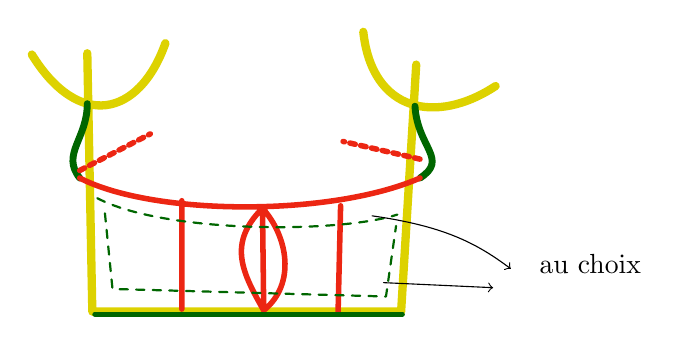
\begin{tikzpicture}[x=.016cm,y=-.016cm,line cap=round,line join=round]
\draw[yellow!70!olive,line width=3pt] (250,767)--(254,972)--(499,972)--(511,776) (206,768)..controls(243,828)and(291,818)..(312,759) (469,750)..controls(476,814)and(527,824)..(574,793);
\draw[black!60!green,line width=2.5pt] (250,807)..controls(250,835)and(229,847)..(244,866) (510,809)..controls(512,842)and(537,851)..(514,866);
\draw[red!70!brown,line width=2pt] (244,866)..controls(302,896)and(443,897)..(514,866) (325,884)--(325,970) (389,890)..controls(361,918)and(373,941)..(390,971)..controls(416,950)and(409,912)..(389,890)--(390,970) (451,888)--(449,972);
\draw[red!70!brown,line width=2pt,dotted] (244,860)--(300,831) (514,851)--(453,837);
\draw[black!60!green,thick,dashed] (258,882)..controls(311,910)and(450,910)..(496,895) (264,894)--(270,954)--(487,960)--(495,904);
\draw[black!60!green,line width=1.8pt] (256,974)--(500,974);
\draw[->] (476,896)..controls(532,904)and(558,917)..(586,938);\draw[->] (485,949)--(572,953);\node[anchor=west] at (601,934) {au choix};
\end{tikzpicture}}

\deleted{c) On trouve} \unsure{au niveau en noir}, \unsure{E}, un \unsure{très} \deleted{\unsure{un}} collier \unsure{strictement canonique} autour de $K$ comme ceci (\unsure{cf. l'isom.} utilisé pour la construction de $\varphi$ au voisinage de $K_0$) et on remplace $F$ par la face \inserted{$F_0^*$} déduite en enlevant $F\cap\mathring C$.

\figure{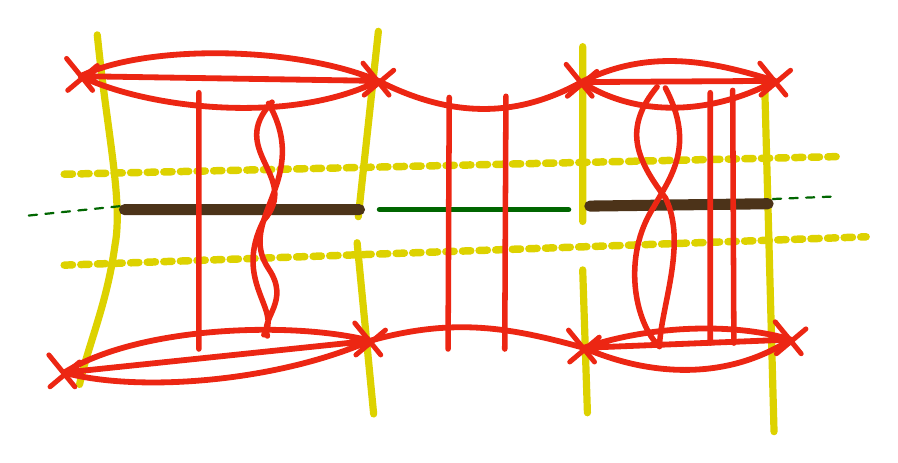
\begin{tikzpicture}[x=.015cm,y=-.015cm,line cap=round,line join=round]
\draw[yellow!70!olive,line width=2.6pt] (239,1504)..controls(247,1585)and(261,1645)..(254,1682)..controls(247,1733)and(231,1767)..(224,1800) (477,1501)--(460,1658) (459,1680)--(473,1825) (650,1514)--(650,1662) (650,1703)--(654,1824) (804,1543)--(812,1840);
\draw[yellow!70!olive,line width=2.7pt,dashed] (211,1622)--(870,1607) (211,1699)--(890,1675);
\draw[black!60!green,thick,dashed] (181,1657)--(259,1649) (811,1643)--(860,1641);
\draw[black!60!brown,line width=4pt] (262,1652)--(461,1652) (656,1649)--(807,1647);
\draw[black!60!green,line width=2pt] (478,1652)--(638,1652);
\draw[red!70!brown,line width=2.1pt] (225,1539)..controls(279,1512)and(407,1513)..(477,1543)..controls(401,1581)and(280,1566)..(225,1539)--(477,1543) (211,1790)..controls(273,1751)and(403,1746)..(470,1763)..controls(390,1798)and(273,1807)..(211,1790)--(470,1763) (477,1543)..controls(538,1574)and(593,1575)..(649,1544) (470,1763)..controls(542,1743)and(589,1752)..(651,1769) (649,1544)..controls(710,1513)and(767,1529)..(813,1543)..controls(763,1570)and(699,1576)..(649,1544)--(813,1543) (651,1769)..controls(714,1748)and(783,1749)..(826,1762)..controls(775,1795)and(711,1795)..(651,1769)--(826,1762);
\draw[red!70!brown,line width=2pt] (325,1553)--(325,1770) (387,1561)..controls(348,1602)and(412,1624)..(380,1661)..controls(353,1713)and(396,1737)..(380,1758) (384,1562)..controls(421,1627)and(356,1660)..(384,1702)..controls(403,1730)and(377,1743)..(383,1759) (537,1557)--(536,1770) (585,1556)--(584,1770) (713,1548)..controls(684,1583)and(695,1609)..(720,1642)..controls(739,1680)and(716,1735)..(715,1768) (720,1549)..controls(746,1598)and(724,1625)..(710,1650)..controls(683,1692)and(694,1748)..(715,1768) (758,1553)--(758,1765) (777,1551)--(778,1765);
\foreach \x/\y in {226/1539,477/1543,649/1544,813/1543,211/1790,470/1763,651/1769,826/1762}\draw[red!70!brown,line width=1.8pt] (\x-13,\y-15)--(\x+9,\y+12) (\x-12,\y+12)--(\x+13,\y-9);
\end{tikzpicture}}

\uline{NB} Ce collier est isomorphe (\unsure{dans la catégorie isotopique considérée}) aux voisinages tubulaires des $\widetilde D_i$ dans $\widetilde X$.

e) Pour les faces exceptionnelles \inserted{$F^a$, \unsure{adjacente|adjacence}: $K_{D_i}$,} on \unsure{retrouve} le système $\Sigma$, \deleted{\unsure{en faisant}} \inserted{affiné} par le choix de $D_i$, en prenant ``la partie de $F^*$ au dessus'' de la pseudo-psdr $\delta$, et faisant les modifications d'usage au voisinage des pts critiques.

\figure{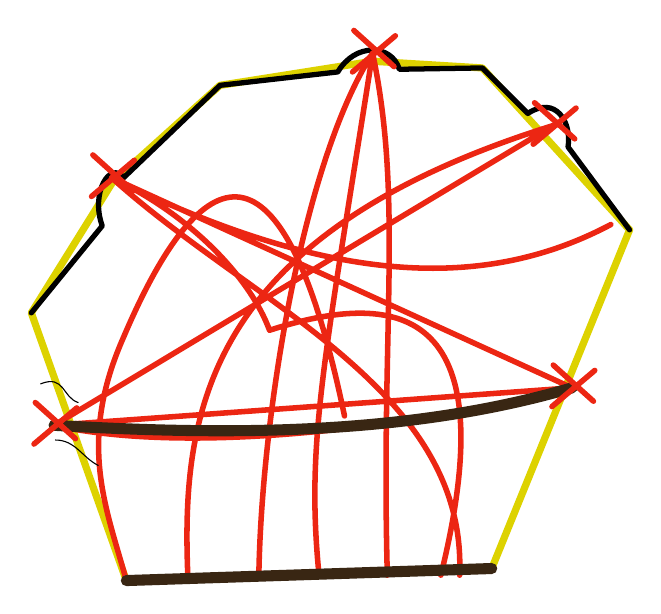
\begin{tikzpicture}[x=.017cm,y=-.017cm,line cap=round,line join=round]
\draw[yellow!70!olive,line width=2.6pt] (1856,1252)--(1785,1052)--(1846,954)--(1926,882)--(2040,864)--(2122,869)--(2232,990)--(2129,1243)--cycle;
\draw[black,line width=1.9pt] (1785,1052)--(1838,987)..controls(1829,962)and(1844,938)..(1854,951)--(1926,882)--(2014,872)..controls(2027,850)and(2054,851)..(2060,870)--(2122,869)--(2156,903)..controls(2177,889)and(2189,910)..(2186,928)--(2232,990);
\draw[red!70!brown,line width=2pt] (1856,1252)..controls(1841,1197)and(1819,1149)..(1854,1070)..controls(1912,934)and(1973,908)..(2019,1129) (1902,1250)..controls(1897,1129)and(1912,994)..(2175,912) (1955,1248)..controls(1957,1128)and(1988,939)..(2040,858) (2000,1248)..controls(1990,1148)and(2004,1088)..(2040,858)..controls(2063,967)and(2046,1064)..(2051,1248) (2091,1248)..controls(2139,1053)and(2065,1032)..(1963,1065)..controls(1949,1027)and(1906,980)..(1845,951) (2105,1248)..controls(2111,1109)and(1950,1046)..(1845,951)..controls(2004,1029)and(2120,1038)..(2218,986) (1802,1136)--(2189,1108) (1802,1136)--(2175,912) (1845,951)--(2189,1108) (1802,1136)..controls(1911,1160)and(2085,1134)..(2189,1108);
\draw[black!70!brown,line width=4pt] (1856,1252)--(2129,1243) (1802,1136)..controls(1924,1143)and(2062,1145)..(2189,1108);
\foreach \x/\y in {1845/951,2040/858,2175/912,1802/1136,2189/1108}\draw[red!70!brown,line width=2pt] (\x-14,\y-17)--(\x+16,\y+10) (\x-15,\y+14)--(\x+17,\y-13);
\draw (1792,1105)..controls(1810,1098)and(1808,1115)..(1820,1119) (1803,1147)..controls(1818,1147)and(1823,1160)..(1835,1166);
\end{tikzpicture}}

f) Attention, à cause de la rectification b), il n'est plus correct de considérer les arêtes exceptionnelles \inserted{de $K$} comme étant celles qui ne contiennent pas des sommets de $L$ (\unsure{et} elles sont exceptionnelles au \unsure{sujet d'une telle propriété}, c'est plutôt qu'elles \uline{peuvent} en contenir plusieurs!). \deleted{Par contre on peut considérer d'autres faces exceptionnelles \unsure{isotopes}, \unsure{en termes}} \inserted{Mais: \unsure{considérons} $K_0'$, comme \unsure{la réunion des|le voisinage plus}} \unsure{comp. connexes|comp. connexe} du $\unsure{K_0'}$ déployement $K'$ qui \uline{n'ont pas de bord global}, d'où un élément très naturel pour introduire ensuite la donnée d).
}
\margin{117}
